\chapter{Zestawienie najważniejszych wariantów zasad gry}
\label{zestawienie_zasad}
\section{Różnorodność zasad gry w madżonga w Chinach i na świecie}
\epigraph{麻将源于中国属于世界 \\ 
\footnotesize \pinyin{Májiàng yuán yú Zhōngguó shǔyú shìjiè} \normalsize \\
Mahjong pochodzi z Chin, lecz
należy do świata.}{Yu Guangyuan\footnote{Yu Guangyuan (于光远 Yú
Guāngyuǎn) (1915-2013) -- znany chiński filozof i działacz Komunistycznej Partii
Chin; prezes Światowej Organizacji Madżonga w latach 2005 do 2013 (Sina
Xīnlàng Lùntán 2010; Wikipedia 2016).}
\\ (Shìjiè Májiàng Zǔzhī 2014)}

Aktualnie na świecie istnieje kilkadziesiąt rozróżnialnych zestawów zasad gry
w madżonga. W wielu przypadkach gracze pochodzący z danego obszaru nie są
nawet świadomi istnienia innych wariantów niż ten, w który grają sami. Według
klasyfikacji Toma Slopera jest ich 42 (Sloper 2002), jednakże nie uwzględnia on
wielu spośród mniej znanych lub różniących się od nich drobnymi szczegółami, jak
choćby odmiana południowoafrykańska (zbliżona do zasad, zgodnie z którymi gra
się w Hongkongu) (World Series of Mahjong 2015).

Warto także wspomnieć, że nawet współcześnie powstają nowe warianty gry, które
cieszą się zainteresowaniem wprowadzając innowacyjne zasady, jednakże przestrzegając w
wystarczającym stopniu tych istniejących wcześniej, aby wciąż klasyfikowano je
jako reguły gry w madżonga. \label{washizu} Przykładem takich zasad jest
japoński madżong \romaji{washizu} (鷲巣), zwany również madżongiem transparentnym
(麻雀透明 \romaji{mājan tōmei}). Pochodzi on z mangi pod tytułem \tytul{,,Akagi:
Geniusz, który zstąpił w ciemność''} (アカギ闇に降り立った天才 \romaji{Akagi:} \romaji{Yami}
\romaji{ni} \romaji{Oritatta} \romaji{Tensai}), która jest wciąż wydawana od
1992 roku przez \mbox{Nobuyuki} \mbox{Fukumoto} (福本伸行 \mbox{Fukumoto}
\mbox{Nobuyuki}).
Esencją sukcesu \romaji{washizu} jest zmiana trzech czwartych kamieni na transparentne, co
drastycznie zmienia przebieg rozgrywki. Pomijając tę zmianę i sposób podziału
kamieni, madżong transparentny w zasadzie nie różni się od japońskich zasad
turniejowych \romaji{rīchi},
% (patrz:strona \pageref{rīchi})
jednakże mimo to stał się on popularny na całym świecie. Podobnych przykładów
powstających współcześnie i zyskujących rozgłos nowych zasad gry w madżonga jest
wiele (Miller 2015).

W związku z mnogością różnorodnych zasad autor nie opisze ich wszystkich w
treści niniejszej pracy, skupiając się na tych z nich, które współcześnie są
najpopularniejsze lub miały historycznie największy wpływ na kulturę gry w
madżonga. Jako punkt odniesienia w ich zestawianiu potraktowane zostaną
międzynarodowe zasady turniejowe, których szczegółowy opis znajduje się w
rozdziale \ref{guobiao}.
%  oraz skróconym
% scharakteryzowaniu 6 innych spośród najpopularniejszych i najbardziej wpływowych
% wariantów (patrz: strona \pageref{inne_zasady}). 

\section{Madżong chiński klasyczny}
\label{cc}
\def \refpodwariantycc {\getrefnumber{podwarianty_cc}} 
%\subsection{Historia}
Na przełomie XIX i XX wieku (patrz: rozdział \ref{historia}) nastąpiło
przekształcenie licznych gier karcianych w pierwsze postaci madżonga. Ze względu
na brak spisanych i ustalonych reguł w tym okresie występowało wiele
rozbieżności w kwestii stosowanych zasad.
Pierwsze próby standaryzacji nastąpiły w latach dwudziestych
XX wieku w Szanghaju (patrz: strona \pageref{shanghai20s}). Naturalnie, pomiędzy
samymi zasadami ustandaryzowanymi przez różnych piszących w tym czasie autorów
również występowały pewne rozbieżności, jednakże wszystkie one są łącznie
określane jako ,,zasady chińskie klasyczne'' (Sloper 2006).

Nie jest pewne, czy zasady klasyczne są najstarszymi zasadami,
choć jest to bardzo prawdopodobne (więcej na ten temat w sekcji \ref{ccvshkos}
na stronie \pageref{ccvshkos}).

Wyjaśnienie najważniejszych, szczególnych cech zasad chińskich klasycznych w
dalszej części tej sekcji wykonane zostało na podstawie ich 3
najważniejszych podwariantów wyszczególnionych w ,,Amerykańskim Kodeksie Praw
Madżonga'' (Babcock \& Foster \& Hartman \& Smith \& Work 1924), nazywanych
dalej (zgodnie z nazewnictwem stosowanym w kodeksie)
\foreign{Mixed-Hand}\footnote{\label{podwarianty_cc}Nazwy 3 wymienionych
podwariantów pochodzą od wymagań narzuconych dla wygrywającej ręki w każdym z
nich. \foreign{Mixed-Hand} to dosłownie ,,mieszana ręka'' (brak restrykcji
względem używanych kamieni), \foreign{One-Double} to ,,jedno podwojenie'' (jeden
obowiązkowy mnożnik na wygrywającej ręce), natomiast \foreign{Cleared-Hand} --
,,wyczyszczona ręka'' (wymagana jest czysta ręka składająca się z tylko jednego
typu kamieni oraz opcjonalnie honorów).},
\foreign{One-Double}\footnotemark[\refpodwariantycc] oraz
\foreign{Cleared-Hand}\footnotemark[\refpodwariantycc].

Wiatr miejsca (a tym samym miejsce przy stole gracza) przydzielany jest poprzez
zmieszanie ze sobą 4 różnych kamieni wiatrów a następnie dobranie po jednym
przez każdego z graczy (osoba mieszająca kamienie bierze ostatni kamień).

\label{cc_mixed_hand}
W czasie konstrukcji muru w podwariancie \foreign{Mixed-Hand} (ale nie w
\foreign{One-Double} oraz \foreign{Cleared-Hand}) z jego części wydzielany jest
tak zwany ,,martwy mur''. Tym mianem określa się 14 kamieni od końca muru, z
których nie można dobierać w procesie gry w zwyczajnym procesie tury, lecz
jedynie jako uzupełnienia kwiatów oraz \pinyin{gangów}. Tym samym, ostatnim
dostępnym kamieniem na potrzeby konkretnych układów jest piętnasty kamień od
końca muru, a nie pierwszy, jak w przypadku międzynarodowych zasad turniejowych.

Zestaw do gry składa się ze 144  lub 136 kamieni (kamienie kwiatów są
opcjonalne -- w przypadku ich braku każdy z boków muru jest o 1 kamień krótszy,
czyli ma długość 17 kamieni). Kamienie kwiatów i pór roku są rozróżniane między
sobą -- zebranie 4 pór roku lub 4 pozostałych kwiatów przez jednego gracza
nazywane jest ,,bukietem''.

Zamiast rotacji miejsc stosowanej w przypadku międzynarodowych zasad
turniejowych, gracze przekazują wiatr miejsca w kierunku przeciwnym do wskazówek
zegara po każdym rozdaniu, w którym nie zwyciężył gracz wschodni (czyli na
początku każdej nowej rundy wiatr wschodni przypisany jest do tego samego
gracza). W przypadku gdy w rozdaniu zwycięży gracz z przypisanym wiatrem
wschodnim, wiatry miejsc nie ulegają przesunięciu i rozgrywane jest dodatkowe
rozdanie (innymi słowy, runda składa się ze zmiennej liczby rozdań -- 4 + liczba
zwycięstw wiatru wschodniego w tej rundzie).

Informacje o kolejności odrzuconych kamieni oraz o pochodzeniu kamieni dobranych
po deklaracjach od innych graczy nie są przechowywane na stole. Odrzucone
kamienie odrzucane są na podłogę pomiędzy ścianami muru w nieuporządkowany
sposób, a w przypadku sekwensów, trójek i \pinyin{gangów} nie ma potrzeby
oznaczania od kogo został dobrany brakujący kamień. 

Układy punktowane dzielą się na podstawowe (które są sumowane przy wygranej)
oraz podwajające. Każdy układ podwajający pozwala przemnożyć sumę punktów
podstawowych przez 2. Innymi słowy, stosowany jest następujący wzór (S -- łączna
wartość ręki; suma -- suma punktów podstawowych; n -- liczba układów
podwajających):
	\begin{equation*}
		S = suma \times 2^n
		\label{zimo}
	\end{equation*}

Wygrywająca ręka, podobnie jak w prawie wszystkich odmianach współczesnego
madżonga, musi składać się z 4 zestawów (trójek, sekwensów lub \pinyin{gangów})
oraz pary. W przypadku najprostszego podwariantu -- \foreign{Mixed-hand} , nie
ma żadnych dalszych restrykcji. \foreign{One-Double} wymaga, aby ręka spełniała co
najmniej jeden z układów podwajających (za wyjątkiem kamieni kwiatów), natomiast
przy \foreign{Cleared-Hand} niezbędne jest, aby ręka używała tylko jednej talii
(z albo bez honorów), samych honorów lub tylko kamieni terminalnych.

Podsumowując, zasady klasyczne zawierają w sobie dużo wyższy czynnik hazardowy,
wygrana jest zdecydowanie bardziej zależna od przypadku, niż ma to miejsce w
przypadku zasad stosowanych współcześnie na zawodach sportowych. Jednakże, wciąż
cieszą się one pewną popularnością, jako że nie są tak skomplikowane, jak wiele
powstałych później wariantów zasad, a wciąż zawierają wszystkie najważniejsze
elementy rozgrywki, przez co często są wykorzystywane jako zasady szkoleniowe.

%TODO: hong kong new style 
\section{Madżong kantoński}
\label{hkos}
Madżong kantoński, znany również jako hongkoński, występuje w 2 różnych
odmianach, zwanych ,,starym stylem'' (lub po prostu ,,starymi zasadami) oraz
,,nowym stylem''.

Nie jest niczym zaskakującym, że na terenie Kantonu (ale nie w Hong Kongu) w
czasie gry używa się kantońskiej wymowy deklaracji, nazw kamieni i układów.
Należy jednakże mieć na uwadze, że nie wszystkie wersje kantońskie są czytaniami
tych samych znaków -- dla przykładu, przy deklaracji \pinyin{chi} w Kantonie
używa się słowa \jyutping{seon} (順 \jyutping{seon6}), a nie \jyutping{hek} (喫
\jyutping{hek3}) (Rep 2006).

Jako że w Hong Kongu hazard nie jest zakazany, madżong kantoński (również w
nowym stylu) nigdy nie utracił cech gry hazardowej. %TODO: źródlo

\subsection{Stary styl}
Wszystkie podwarianty zasad popularne aż do lat czterdziestych XX wieku (do
wybuchu II Wojny Światowej) na terenie Kantonu zaliczane są do starych zasad.
Jako że w przeciwieństwie do zasad klasycznych (oraz ich późniejszej wariacji --
nowego stylu) nigdy nie zostały one ustandaryzowane, występuje wiele
pomniejszych różnic pomiędzy różnymi postaciami tych reguł (zazwyczaj dotyczą
one punktacji pomniejszych układów i wypłat przy zakończeniu rozgrywki). Przez
długi czas były one w użyciu równolegle z zasadami klasycznymi, w związku z czym
widocznych jest pomiędzy nimi wiele podobieństw (Depaulis [\&] Tsui 2007).

Wiele wskazuje na to, że ten zestaw zasad jest nie tylko jednym ze starszych,
ale wręcz jest najstarszym ze wszystkich, choć wciąż jest to przedmiotem
nierozstrzygniętej dyskusji (więcej na ten temat w sekcji \ref{ccvshkos} na
stronie \pageref{ccvshkos}). Do dzisiaj jest on rozpowszechniony nie tylko w
Kantonie i Hong Kongu, lecz na całym świecie.

Sam proces gry różni się jedynie detalami od madżonga klasycznego.
Przykładowo, zakryty \pinyin{gang} po deklaracji składa się (wbrew nazwie) z
odkrytych kamieni (podczas gdy w madżongu klasycznym i większości innych
odmian, tylko 2 wewnętrzne kamienie są odkryte, natomiast zgodnie z
międzynarodowymi zasadami turniejowymi wszystkie 4 kamienie muszą być zakryte
-- patrz: Rysunek \ref{fig:closed_gang_options} oraz zasady międzynarodowe
turniejowe na stronie \pageref{closed_gang}).
Występuje więcej podobnych, drobnych różnic, lecz w większości nie mają one dużego wpływu na przebieg
rozgrywki.

\begin{figure}[H]
  \centering
  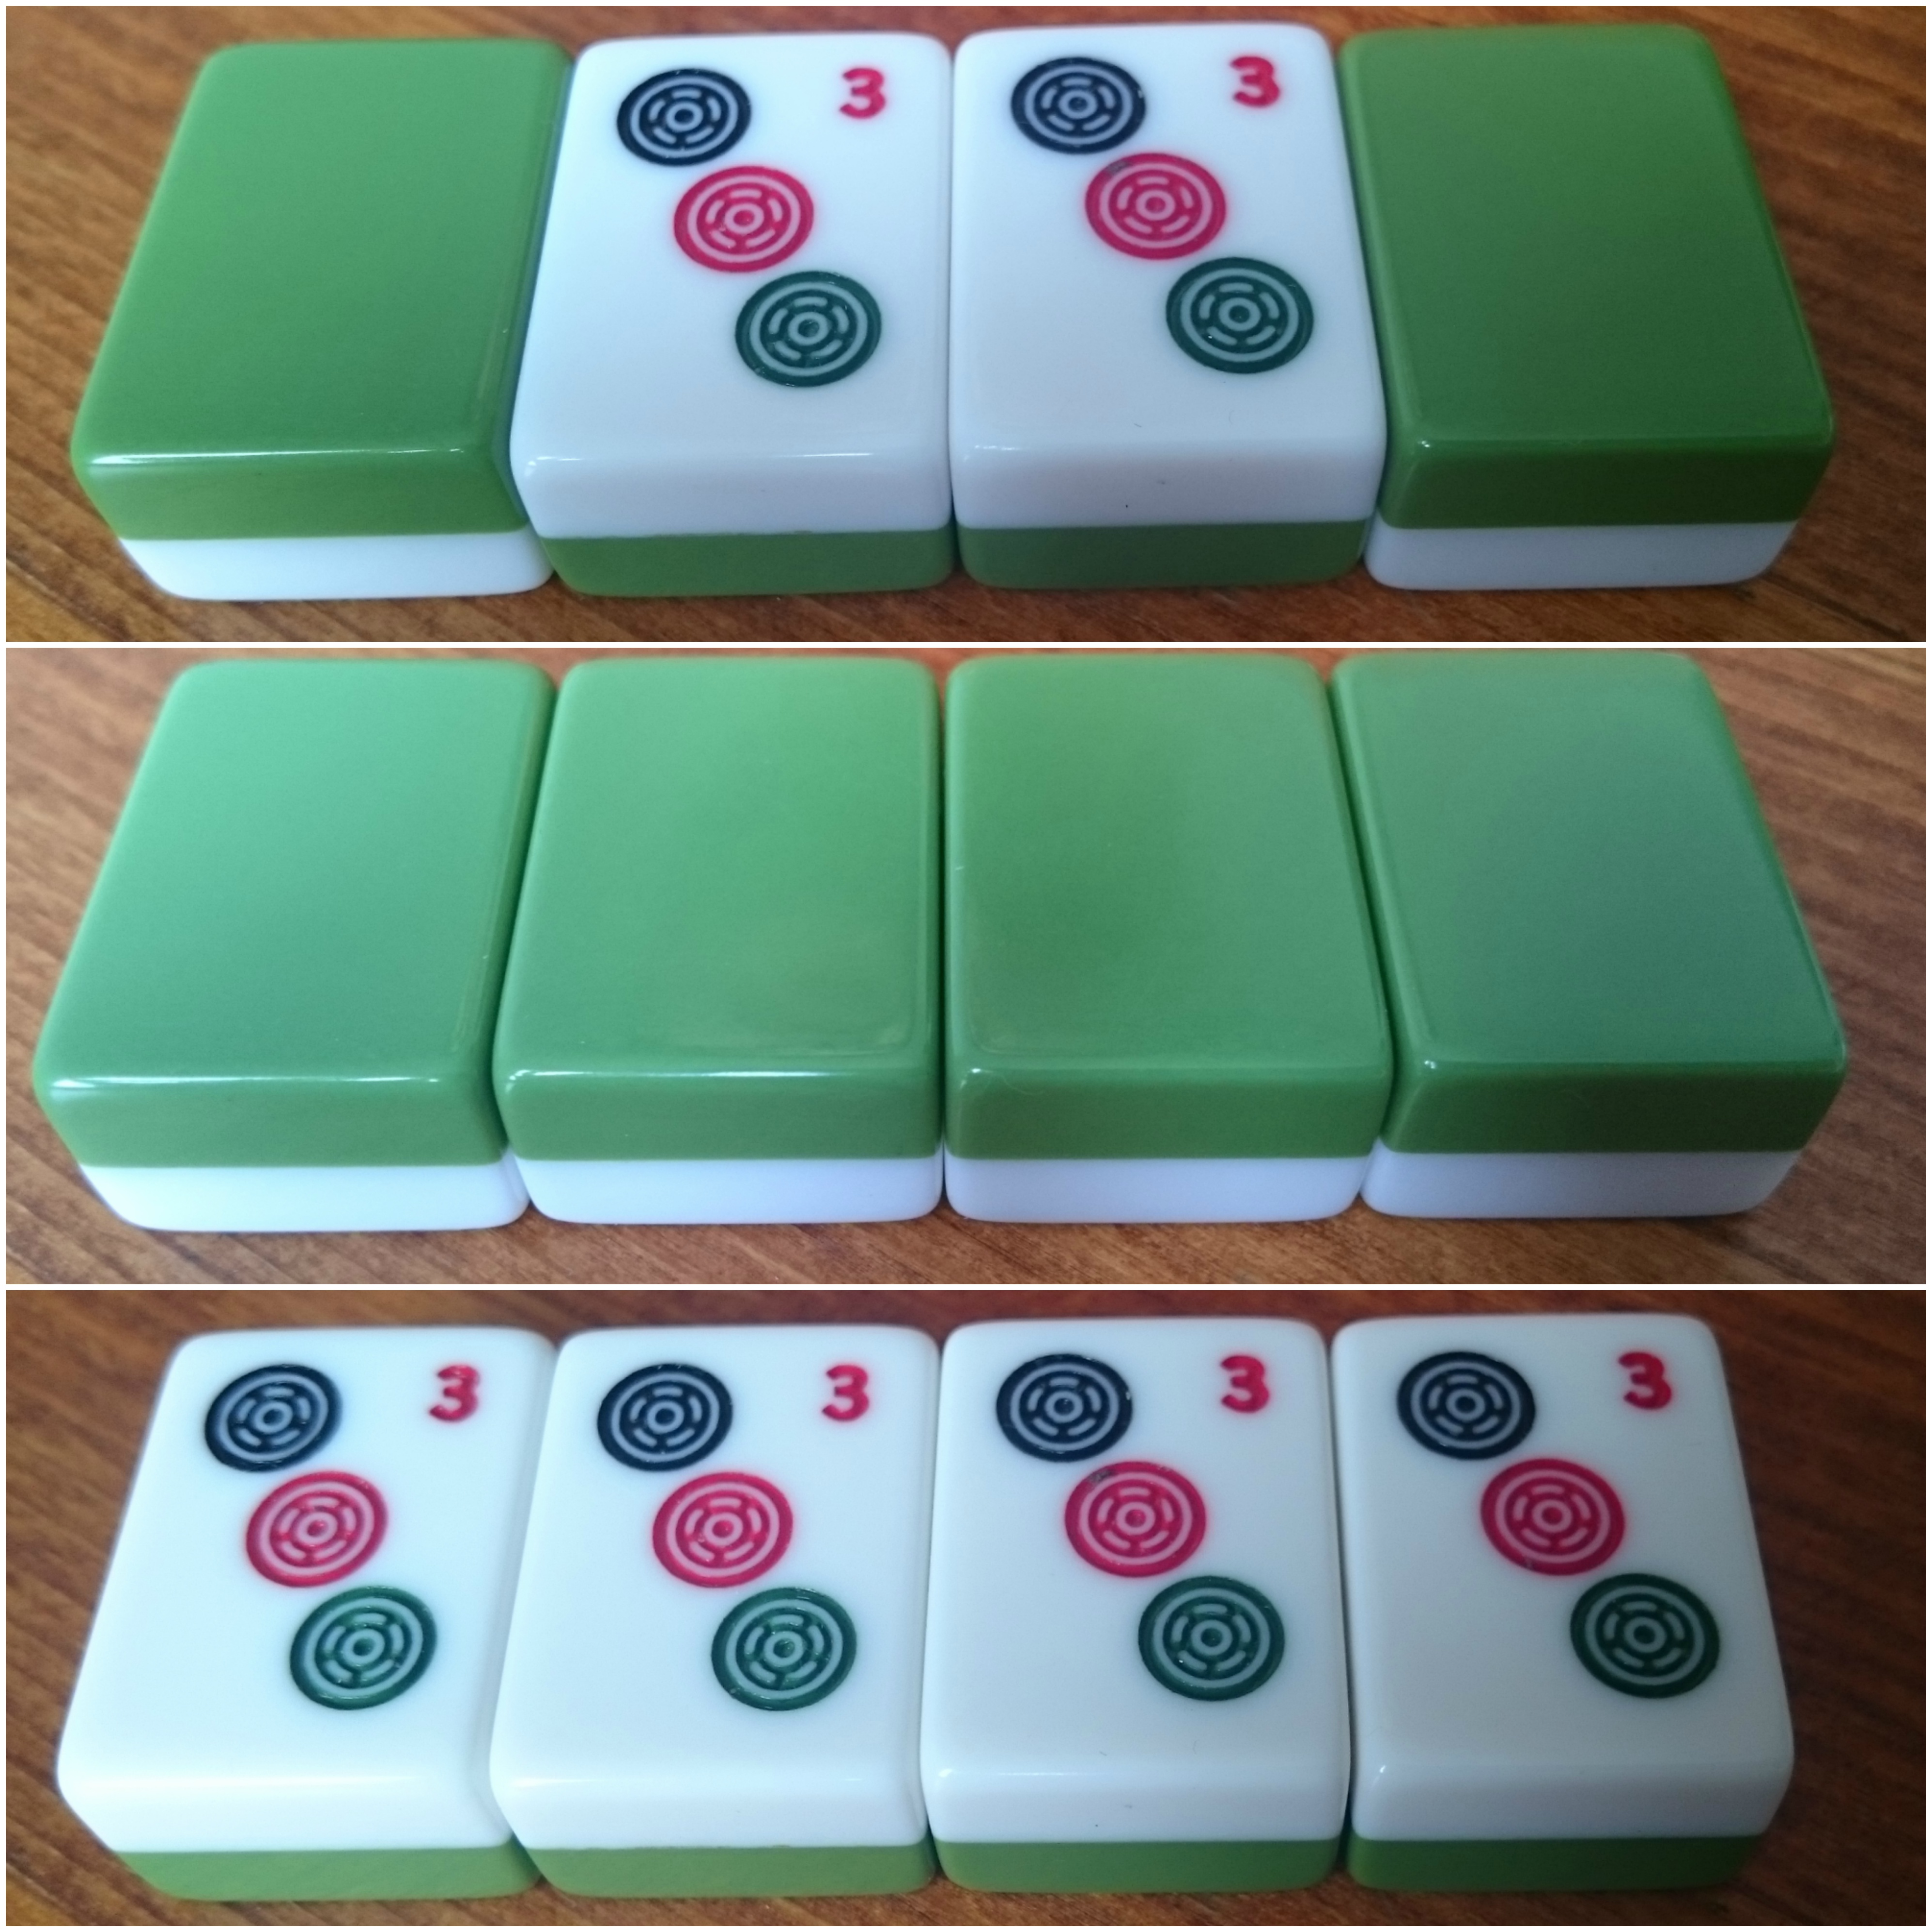
\includegraphics[width=0.50\textwidth]{gang_wariacje.jpg}
  \caption{3 możliwości oznaczania zamkniętego \pinyin{ganga}; kolejno od góry:
  w madżongu klasycznym i \romaji{rīchi}; w międzynarodowych zasadach
  turniejowych i w madżongu kantońskim; źródło: fotografia własna}
  \label{fig:closed_gang_options}
\end{figure}

Elementem wyróżniającym jest natomiast system liczenia punktów, który podobnie
jak międzynarodowe zasady turniejowe, oparty jest o \pinyin{fan} (jednakże
nie wszystkie układy i ich wartości są takie same - patrz też: strona
\pageref{fan}). Zsumowana wartość \pinyin{fan} jest traktowana jako wykładnik
potęgi liczby 2 przy liczeniu wartości punktowej ręki, zgodnie ze wzorem(S --
łączna wartość ręki; p - łączna wartość \pinyin{fan}):
	\begin{equation*}
		S = 2^{p}
		\label{hkos_scoring:point_score}
	\end{equation*}
Łączna wartość fan to wspomniana suma, zgodnie ze wzorem (f -- wartość danego
\pinyin{fan}; n -- liczba wszystkich \pinyin{fan}, które wystąpiły na
wygrywającej ręce):
	\begin{equation*}
		p = \sum\limits_{i=1}^n f_{i}
		\label{hkos_scoring:fan_score}
	\end{equation*}
(Lo 2001)

\subsection{Nowy styl}
Nowy styl wariantu kantońskiego to jego młodsza odmiana, która stała się
popularna po II Wojnie Światowej. Później, gdy w 1966 w Chińskiej Republice
Ludowej zakazano gry w madżonga, wielu udawało się do Hong Kongu tylko po to, by
móc grać - a nowy styl był tam najpopularniejszym zestawem zasad (Rep 2006).

Nowy styl stał się również niezwykle popularny w Szanghaju, przez co można się
też spotkać z nazywaniem go ,,madżongiem szanghajskim'' (Miller 2013).

Już od początku rozgrywki widać wizualne różnice. Mur budowany jest w inny
sposób -- zamiast kłaść kamienie na sobie w 2 warstwach, są one umieszczane
równolegle obok siebie (lub w kształt ,,wiatraka'' -- patrz: Rysunek
\ref{fig:hkns_wall}).

\begin{figure}[H]
  \centering
  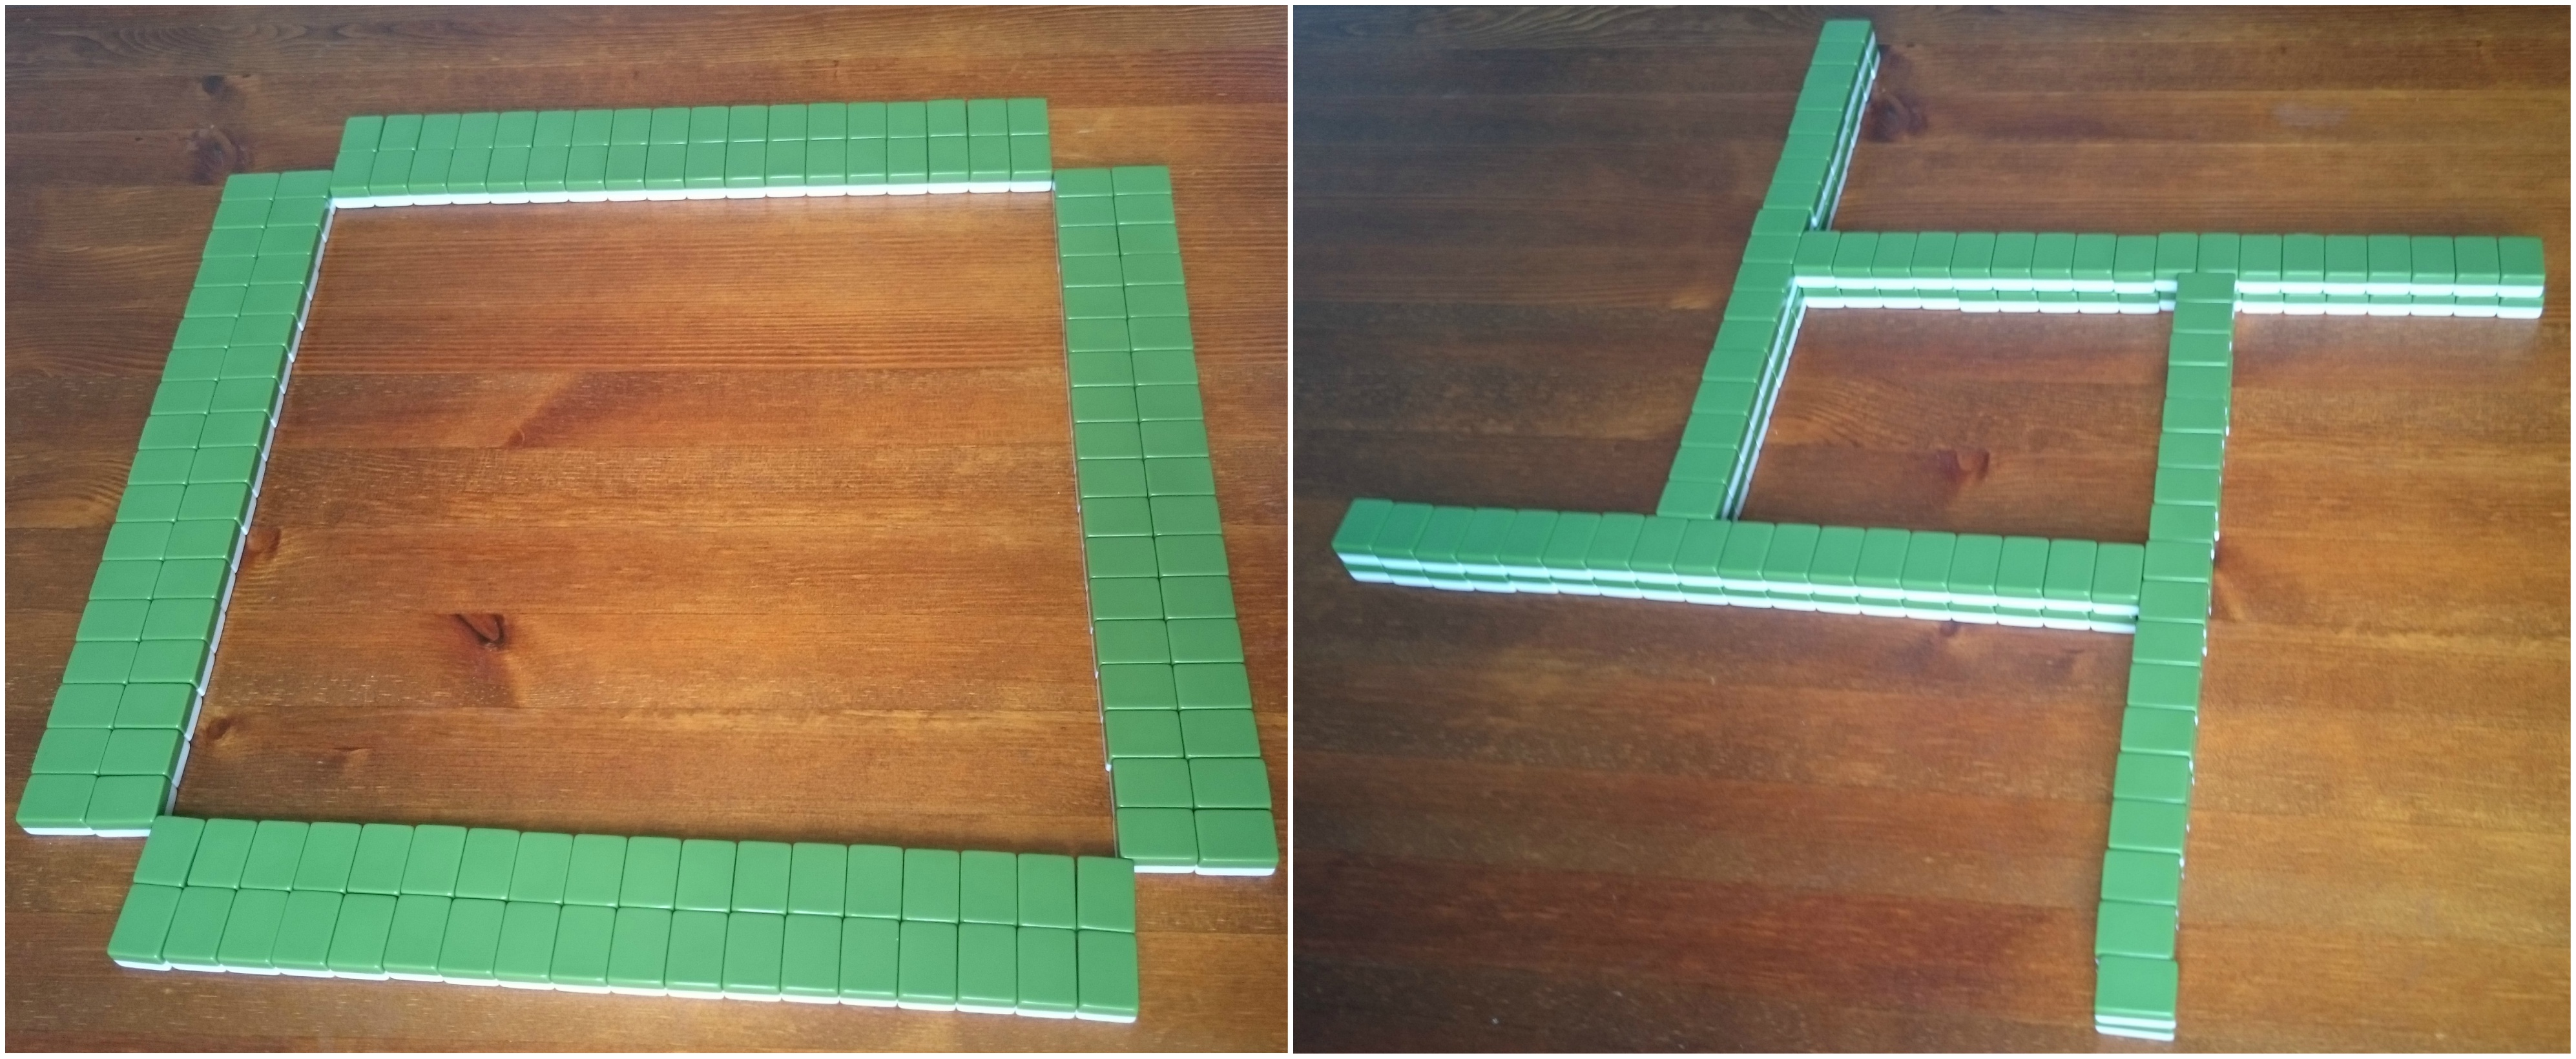
\includegraphics[width=0.8\textwidth]{hkns_wall.jpg}
  \caption{2 dopuszczalne możliwości budowania muru w nowym stylu madżonga
  kantońskiego; wariant płaski -- kamienie są najpierw
dobierane z wewnętrznego kręgu, a potem z zewnętrznego, naprzemiennie);
,,wiatrak'' -- wraz z postępem gry, mury są spychane do środka stołu, aby
kolejny kamień był łatwy do dobrania dla każdego z 4 graczy; źródło:
  fotografia własna}
  \label{fig:hkns_wall}
\end{figure}

Również przełamanie muru następuje w charakterystyczny sposób - wykonywany jest
tylko jeden rzut, lecz używa się do niego 3 (a nie 2) sześciennych kości.
Ponadto, dokonuje go gracz wschodni i żaden z pozostałych graczy nie bierze
udziału w tej czynności.

System liczenia punktów jest oparty o ten używany w starym stylu, jednakże
używany jest inny (większy) zbiór różnych \pinyin{fan} oraz wprowadzono w nim
limity -- \jyutping{laat} (辣 \jyutping{laat6}). Jako że madżong kantoński jest
grą hazardową, a punkty przeliczane są bezpośrednio na pieniądze, w kontekście
ilości różnych \pinyin{fan}, jakie naraz mogą znaleźć się w tym wariancie na
wygrywającej ręce, wysokie wygrane mogły potencjalnie przekraczać możliwości finansowe
przegranych uczestników gry. Z tego właśnie względu wprowadzono \jyutping{laat},
które pozwalają ograniczyć maksymalną możliwą wygraną. \pinyin{Fan} o łącznej
wartości 4, 5 lub 6 mają wartość 1 \jyutping{laat}, które przekłada się na 16 punktów
(czyli standardową wartość dla 4 \pinyin{fan}). 2 \jyutping{laat} to od 7 do 9
\pinyin{fan}, natomiast 3 \jyutping{laat} to 10 i więcej. W bardziej hazardowym
podwariancie można grać aż do 5 \jyutping{laat} (20 \pinyin{fan}), w czego
efekcie wartość ręki może osiągnąć nawet 2048 punktów, przez co przed grą
istotne jest ustalenie przez graczy, do którego limitu zamierzają grać (Rep 2006).

\section{Wiek madżonga klasycznego i kantońskiego}
\label{ccvshkos}
Niewątpliwie madżong klasyczny oraz kantoński w starym stylu sa najstarszymi
znanymi regułami gry, jednakże jest kwestią sporną, który z nich jest starszy
od drugiego. Argumenty za oboma potencjalnymi rozwiązaniami, które autor
przedstawia w dalszej części tej sekcji, pochodzą z zapisu dyskusji Toma
Slopera, Alana Kwaana i Cofa Tsui (Sloper i inni autorzy 2006).

Za starszeństwem zasad klasycznych przemawia fakt, że wszystkie źródła
pochodzące z lat dwudziestych XX wieku, kiedy zasady gry ulegały standaryzacji,
nie wspominają o wariancie kantońskim, nawet w kontekście Hong Kongu,
co jasno sugeruje, że wariant klasyczny mógł być wówczas jedynym istniejącym.
Ponadto, oba zestawy zasad są bardzo zbliżone w kwestii samego procesu gry,
różniąc się przede wszystkim sposobem liczenia punktów, który z kolei jest mniej
skomplikowany w przypadku madżonga kantońskiego -- z czego można wysunąć
wniosek, że jest on uproszczeniem wersji klasycznej.

Jako że madżong nie powstał od razu w swojej docelowej formie, lecz stanowił
rozwinięcie wielu istniejących wcześniej gier, problem jest tym bardziej
skomplikowany. Ponadto, Cofa Tsui argumentuje, że jest mało prawdopodobne, by w
tak wczesnym okresie rozwoju gry zasady były upraszczane -- naturalnym
kierunkiem rozwoju zasad jest proces odwrotny, co wskazywałoby na starszeństwo
reguł kantońskich.

Zasady kantońskie w przeciwieństwie do klasycznych nie przewidują, aby w
przypadku zwycięstwa w rozdaniu kiedykolwiek któryś z graczy poza wygranym
otrzymywał punkty -- co jest cechą wspólną z \pinyin{madiao} i innymi
protoplastami madżonga. 

Jednakże, zgodnie z badaniami Thierry'ego Depaulisa i Cofa Tsui, istnieje też
teoria, że w rzeczywistości wcześniej (pomiędzy powstaniem gry a 1920 rokiem)
mogło istnieć wiele innych, jeszcze nieustandaryzowanych i niejednolitych
zestawów zasad, z których mogły się wywodzić oba późniejsze warianty (zarówno
klasyczny, jak i kantoński) (Depaulis [\&] Tsui 2007).

\section{Madżong japoński}
Madżong pojawił się po raz pierwszy w Japonii w 1907 roku. Został przywieziony
przez japońskiego żołnierza nazwiskiem Hirayama Saburo, który wcześniej spotkał
się z nim w Chinach, a następnie w roku 1924 założył szkołę gry (w tym samym
roku miały miejsce pierwsze zawody na skalę ogólnokrajową). Według innej teorii
madżong dotarł do Japonii za pośrednictwem pisarza Natsume Sōseki
\footnote{Natsume Sōseki (夏目漱石, 1867-1916) -- jego prawdziwe imię to Kinnosuke
(金之助); pisarz japoński tworzący w epoce Meiji (明治).} -- madżong pojawił się w
zapiskach z jego podróży do Chin w 1909 roku. W ciągu kolejnych dekad nastąpił
gwałtowny wzrost popularności gry w Japonii, grywał w nią nawet sam cesarz
Hirohito (裕仁). W czasie drugiej wojny chińsko-japońskiej\footnote{Druga wojna
chińsko-japońska (1937-1945) -- konflikt pomiędzy Republiką Chińską a Japonią,
którego czas trwania częściowo pokrywa się z II Wojną Światową. Zakończył się
kapitulacją Japonii w 1945 roku.} gra była zabroniona, jednakże zapotrzebowanie
było tak duże, że grano w nią pod fałszywą nazwą \romaji{takugi} (たくぎ). Po
wojnie gra stała się jeszcze bardziej popularna w związku ze zniesieniem zakazu
i pojawieniem się wariantu \romaji{rīchi} (patrz: sekcja \ref{rīchi}) (Kolenda 
2012).

Madżong, podobnie jak znacznie wcześniej pismo chińskie, został przez
Japończyków zaadaptowany do ich potrzeb, zamiast być przyjętym w niezmienionej
postaci. Poza tym, że przy stole używana jest terminologia po japońsku (dla
przykładu, \romaji{kan} (槓 lub カン) zamiast \pinyin{gang}), zestaw do gry różni
się od tego stosowanego w innych wariantach gry. Kamienie kwiatów nie są używane
(większość japońskich zestawów jest ich w ogóle pozbawiona), natomiast
występują 3 unikalne, występujące w jednym egzemplarzu kamienie -- tak zwane
,,czerwone piątki'' lub ,,czerwone \romaji{dory}'' (赤牌 \romaji{akapai} lub 赤ドラ
\romaji{akadora}). Są to dodatkowe egzemplarze kamieni o numerze 5 w każdej z 3
talii, które od zwyczajnych różnią się pomalowanym na kolor czerwony wzorem.
Kamienie białego smoka również różnią się od chińskich - są to białe, gładkie
kamienie bez żadnego wzoru (podczas gdy chiński wzór to czarna lub niebieska
obwódka wokół prostokątnego kamienia) (Rep 2006).

Istnieją 2 główne odmiany madżonga japońskiego -- tradycyjny i \romaji{rīchi}
(立直 lub リーチ) (Kolenda 2012), jednakże ze względu na ogólnoświatową popularność
wariantu \romaji{rīchi} autor postanowił skupić na nim całą uwagę.
% 
% \subsection{Madżong japoński tradycyjny}
% \label{japanese_traditional}

\subsection{Madżong japoński \romaji{rīchi}}
\label{rīchi}
Madżong \romaji{rīchi} powstał w latach pięćdziesiątych XX wieku, kiedy grywali
w niego zawodowi hazardziści, którzy później przyczynili się do jego
popularyzacji. Jest on bardzo popularny nie tylko w Japonii, ale też na
całym świecie (Rep 2006). W samej Japonii żyje ponad 30 milionów graczy, którzy
mogą poświęcać czas swojej pasji w ponad 10 tysiącach wyspecjalizowanych w tego
rodzaju rozrywce lokali (Miller 2015).
Jest to jeden z 2 wariantów zasad gry, zgodnie z którym organizowane są turnieje
Europejskiej Organizacji Mahjonga (drugi to międzynarodowe zasady turniejowe)
(European Mahjong Association 2016) oraz jedyny, w którym organizowane są
turnieje w Polsce (Polska Liga Mahjonga 2016).
Znajdujące się w dalszej części tej sekcji wyjaśnienie wyróżniających elementów
jego zasad zostało wykonane na podstawie aktualnej wersji reguł obowiązujących
na zawodach Europejskiej Organizacji Mahjonga (European Mahjong Association
2016), ich poprzedniej edycji z roku 2012 (European Mahjong Association 2012)
oraz książki \textit{The Great Mah Jong Book: History, Lore, and Play} (Rep
2006). Używana terminologia oparta jest o tę używaną przez Polską Ligę Mahjonga
(Polska Liga Mahjonga 2016).

Istotną częścią zestawu do gry w \romaji{rīchi} są  \romaji{tenbō} (点棒) --
liczmany służące nie tylko do oznaczania posiadanej liczby punktów, ale są też
potrzebne do niektórych sytuacji w grze. Niejako podkreślają też hazardowe
pochodzenie gry, jako że mogą nasuwać skojarzenia z żetonami używanymi w grach
takich jak poker.

Budowa muru na początku rozgrywki jest zbliżona do wariantu \foreign{Mixed-Hand}
zasad chińskich klasycznych (patrz: strona \pageref{cc_mixed_hand}) --
występuje martwy mur składający się ze stałej liczby 14 kamieni. Gdy dobrany
zostanie kamień uzupełniający (嶺上牌 \romaji{rinshanpai} -- dosłownie ,,kamień ze
szczytu góry''), dokładany jest dodatkowy kamień z końca zwykłego muru aby
zachować stałą liczbę kamieni -- w ten sposób dobranie kamienia uzupełniającego
nie wydłuża faktycznie rozgrywki.

Elementem charakterystycznym dla \romaji{rīchi}, którego oznaczenie znajduje się
także w budowie martwego muru, jest \romaji{dora} (ドラ) -- specjalny, losowy w
każdym rozdaniu kamień, którego każde wystąpienie na wygrywającej ręce zwiększa
znacząco jej wartość punktową. To, który kamień jest \romaji{dorą} w danym
rozdaniu, zależy od jej indykatora -- trzeciego kamienia od końca martwego muru.
Jest on odkrywany po zbudowaniu muru, a kamień o wartości o jeden wyższej od
indykatora jest \romaji{dorą} w tym rozdaniu. Ponadto, każda deklaracja
\pinyin{ganga} w rozdaniu wiąże się z odkryciem kolejnego indykatora po jego
lewej stronie, w efekcie czego naraz może być w grze 5 różnych \romaji{dor},
jako że nie jest dozwolone zadeklarowanie więcej niż 4 \pinyin{gangów} w jednym
rozdaniu (patrz: Rysunek \ref{fig:rīchi_dead_wall}).

\begin{figure}[H]
  \centering
  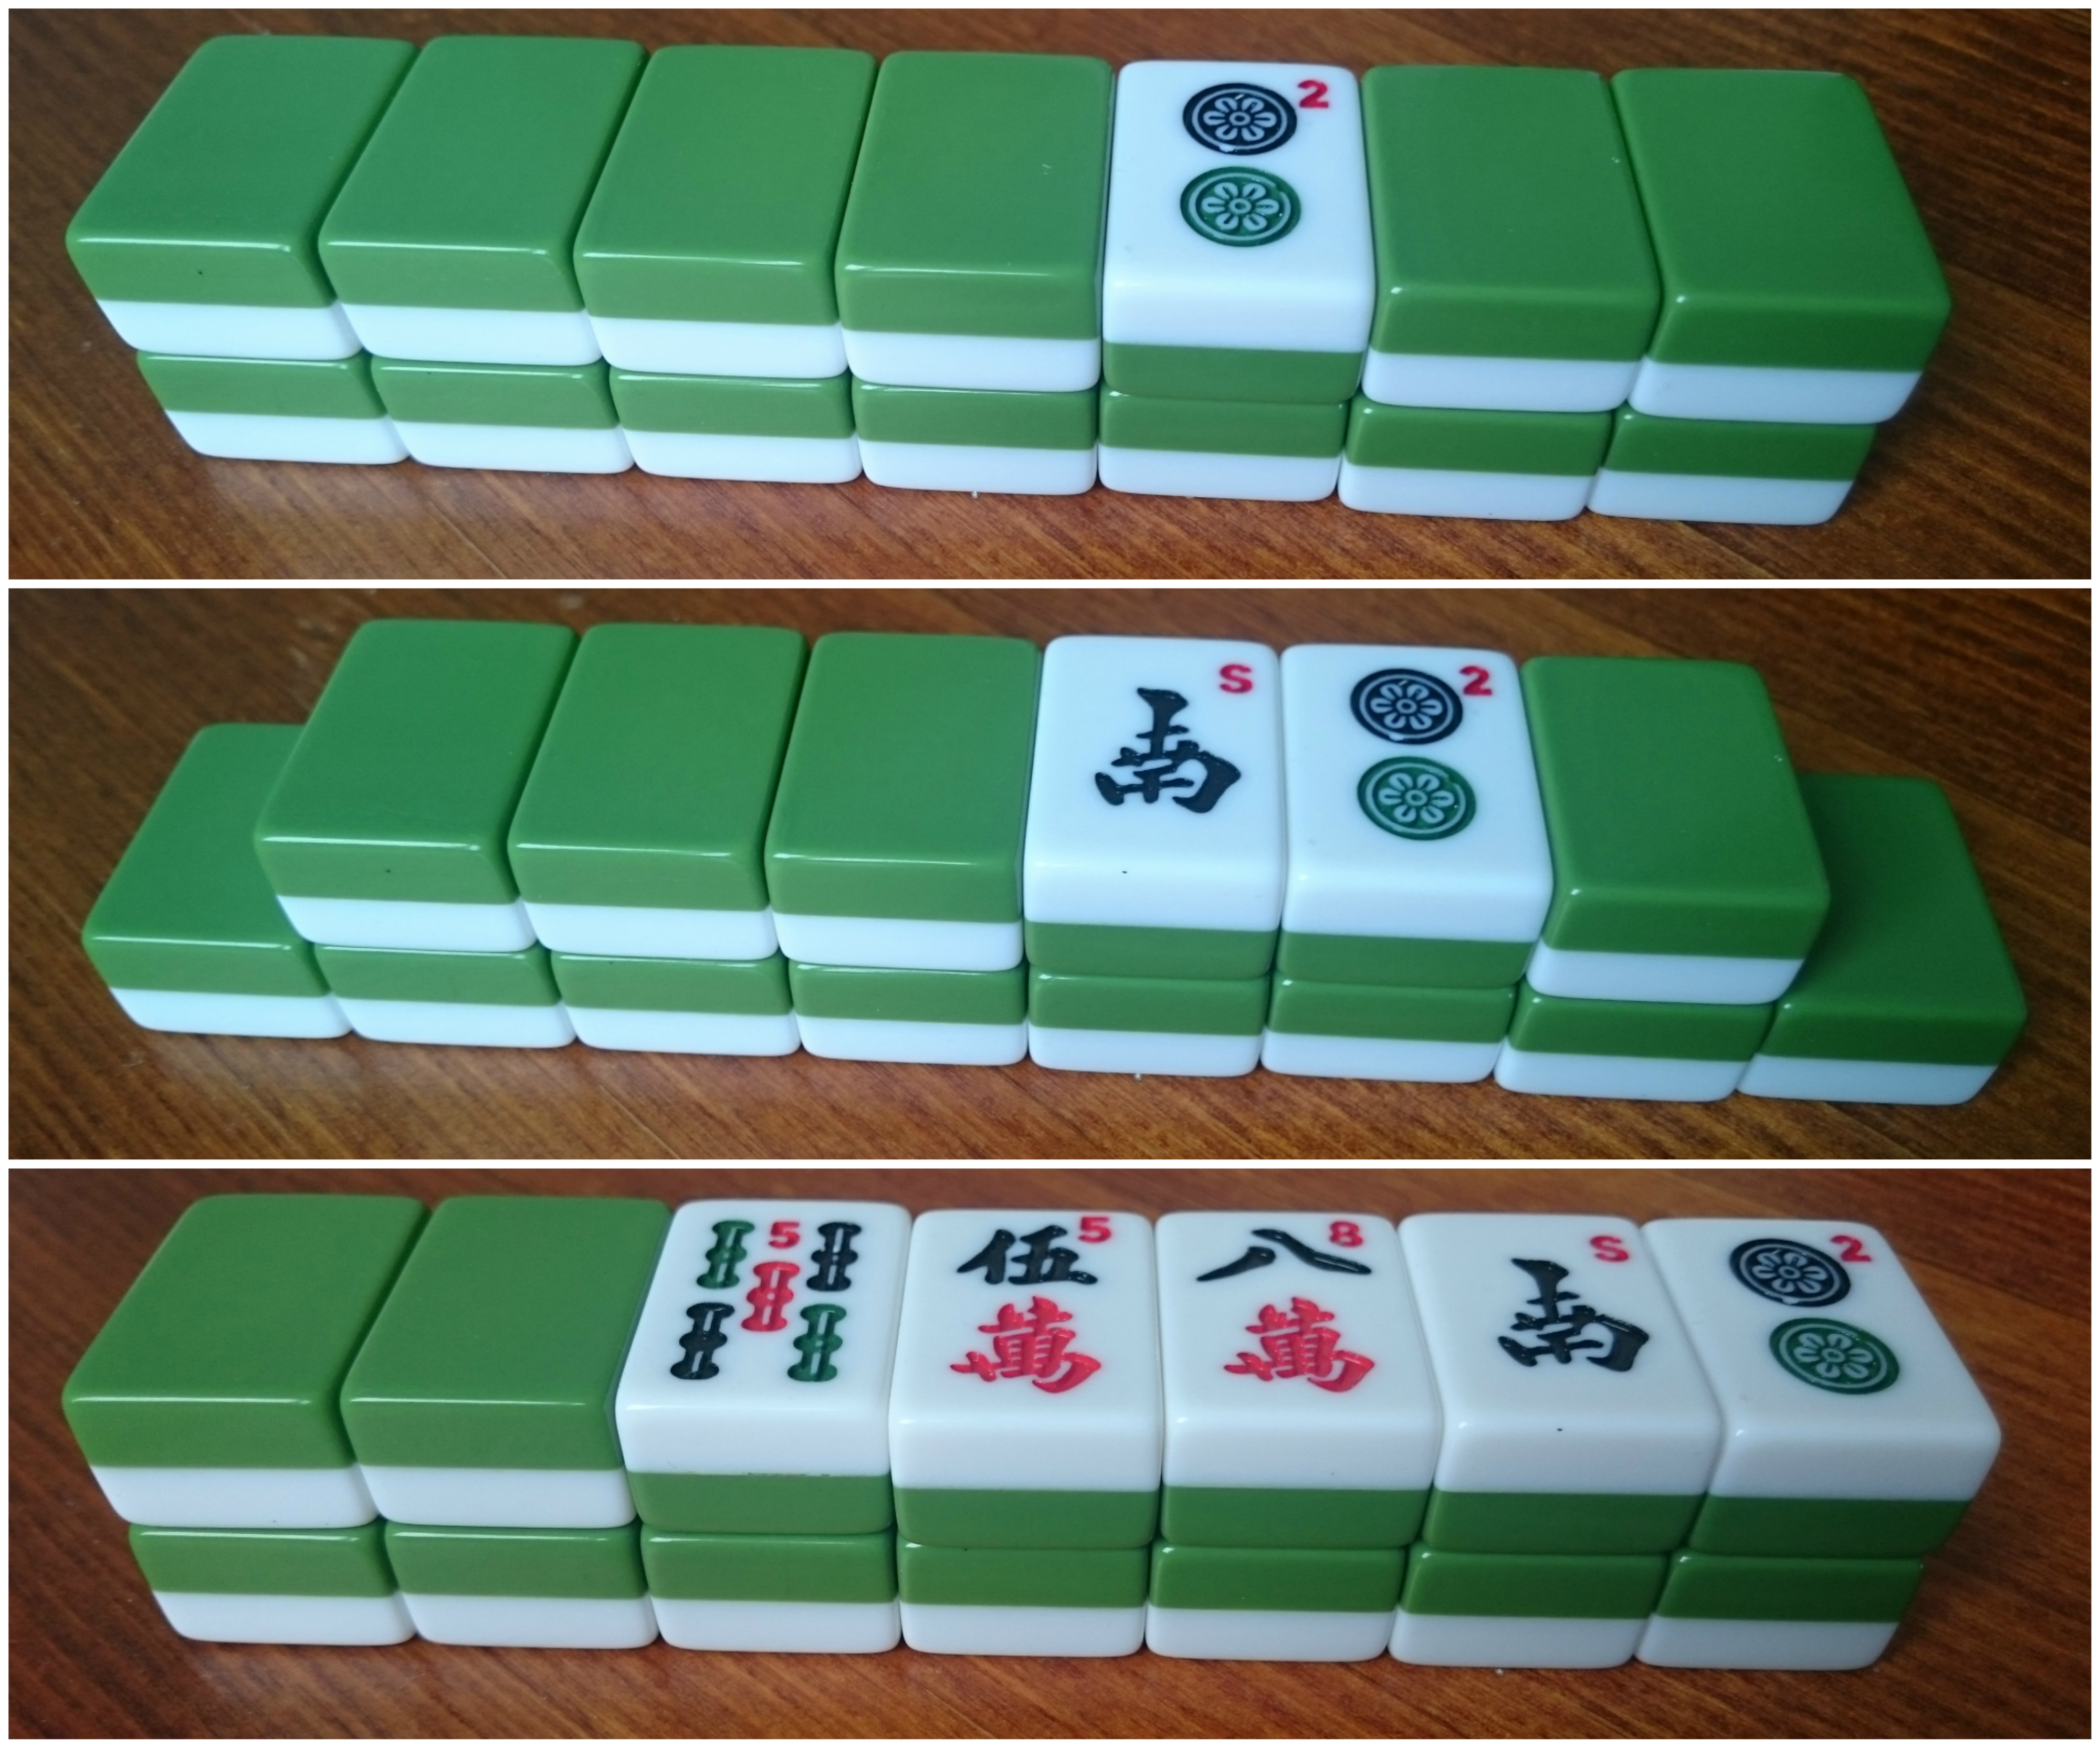
\includegraphics[width=0.5\textwidth]{riichi_dead_wall.jpg}
  \caption{Martwy mur w madżongu japońskim \romaji{rīchi}; indykatorami
  \romaji{dory} są odkryte kamienie, natomiast po ich prawej stronie
  znajdują się kamienie uzupełniające (maksymalnie 4); pierwsza fotografia
  przedstawia stan na początku rozdania, druga -- po deklaracji 1
  \pinyin{ganga}, a trzecia -- po deklaracji wszystkich 4 możliwych
  \pinyin{gangów}; na przykładzie pierwszej fotografii, indykatorem
  \romaji{dory} jest 2 z talii kółek, więc \romaji{dorą} jest 3 z tej samej
  talii; źródło: fotografia własna}
  \label{fig:rīchi_dead_wall}
\end{figure}

Opcjonalną zasadą jest używanie wspomnianych wcześniej czerwonych \romaji{dor}
-- wówczas w każdej talii 1 z 4 kamieni o numerze 5 jest pomalowany wyłącznie
kolorem czerwonym. Czerwone \romaji{dory} są traktowane na
wygrywającej ręce identycznie jak zwykłe. Choć czerwone piątki są standardowym
elementem zestawów do japońskiego madżonga, nie są używane w aktualnej (z 2016
roku) wersji zasad Europejskiej Organizacji Madżonga (jednakże obowiązywały w
wersji z 2012 roku).

Kolejnym elementem charakterystycznym \romaji{rīchi} jest zasada, od której
pochodzi nazwa tego wariantu. \romaji{Rīchi} to specjalna deklaracja dozwolona
wtedy, gdy gracz znajdzie się w stanie czekania (określanym \romaji{tenpai}
(聴牌)) na zakrytej ręce. Wówczas poprzez tę deklarację może zastawić tysiąc
swoich punktów (kładąc odpowiednie \romaji{tenbō} na stół) i umieścić
odrzucony kamień poziomo. Od tego momentu gracz nie może już wykonywać innych
deklaracji (nie licząc zakrytego \pinyin{ganga}, o ile nie zmienia on kamieni,
na które oczekuje gracz) ani zmieniać składu swojej ręki, jednakże wartość
punktowa jego ręki w przypadku wygranej się zwiększy (w przypadku przegranej
1000 punktów, które zostało położone w zastaw na stole, zostaje utracone).

Występuje szereg pomniejszych wyróżniających zasad odróżniających \romaji{rīchi}
od innych wariantów madżonga (zakryty \pinyin{gang} oznaczany jest tak, jak w
zasadach chińskich klasycznych, występuje ścisłe rozróżnienie deklaracji
zwycięstwa na odrzuconym kamieniu oraz na kamieniu dobranym z muru, a także
inne), jednakże pozostałe elementy gry są bardzo zbliżone do madżonga
kantońskiego w nowym stylu. Informacje o odrzuconych kamieniach są zachowywane
na stole, identycznie jak w wyżej wymienionym wariancie, jak też i w
międzynarodowych zasadach turniejowych, jednakże rotacja miejsc na końcu rund
upodabnia te zasady do reguł hongkońskich.

Również system punktacji nasuwa bliskie skojarzenia z zasadami kantońskimi.
Występują limity podobne do \jyutping{laat} przy konkretnych wartościach
punktowych, przy czym każdy z nich ma swoją własną nazwę. 
% (\romaji{mangan},
% \romaji{haneman}, \romaji{baiman}, \romaji{sanbaiman} i \romaji{yakuman})
Istnieją 2 pośrednie rodzaje punktów:
\begin{itemize}
  \item \romaji{han} (飜) -- wartości konkretnych \pinyin{fan}, zwanych w
  madżongu japońskim \romaji{yaku} (役);
  \item \romaji{fu} (符) -- liczone są w bardzo podobny
sposób do punktów podstawowych w madżongu chińskim klasycznym, jak też i pełnią
podobną rolę, będąc wartością mnożoną przez konkretną potęgę liczby 2.
\end{itemize}
Punkty (nie licząc sytuacji, gdy przekraczają któryś z 5 istniejących w
zasadach limitów i są ustaloną wartością) są liczone z następującego wzoru (S
-- łączna wartość punktowa wygrywającej ręki; Fu -- liczba punktów \romaji{fu};
Han -- liczba punktów \romaji{han}):

	\begin{equation*}
		S = Fu \times 2^{2 + Han}
		\label{rīchi_scoring}
	\end{equation*}
	
W przypadku zwycięstwa na kamieniu odrzuconym przez innego gracza, ów gracz jest
odpowiedzialny w pełni za wypłatę wygranej, co narzuca konieczność rozwagi przy
odrzucaniu kamieni (jako że można spowodować nie tylko cudzą wygraną, ale także
utratę własnych punktów) i często -- grę defensywną. Ponadto, wiele
obowiązujących \romaji{yaku} narzuca konieczność posiadania zakrytej ręki, przez
co deklaracje na kamieniach odrzuconych przez innych graczy do własnych zestawów
często nie są tak opłacalne, jak byłoby w innych wariantach zasad.

Mimo że \romaji{rīchi} jest jednym z najbardziej skomplikowanych wariantów, jest
ceniony na całym świecie za swoją dynamikę gry wprowadzaną przez unikalne dla
niego zasady. 

\section{Madżong amerykański}
\label{AMJ}
Podczas gdy w Japonii i Hong Kongu zasady madżonga stawały się coraz bardziej
skomplikowane, w Stanach Zjednoczonych powstawał wariant o zupełnie innej
charakterystyce. W latach dwudziestych i trzydziestych XX wieku gra stanowiła
formę wspólnej rozgrywki łączącej przedstawicieli różnych pokoleń pośród
Chińskich imigrantów w Ameryce. Wspólne rozgrywki w madżonga pomagały im
zachować tożsamość kulturową i wypełniać czas wolny. Zwyczaj ten został również
zaadoptowany przez społeczeństwa innej grupy etnicznej -- imigrantów żydowskich.
To właśnie w ich kręgach reguły gry zostały zmienione do postaci, którą
współcześnie określa się mianem madżonga amerykańskiego lub rzadziej --
madżonga żydowskiego. Stał się on szczególnie popularny pośród kobiet z rodzin,
które wyprowadzały się z miast. Już w latach sześćdziesiątych utrwalony był
(często krzywdzący) stereotyp żydowskiej gospodyni grającej w madżonga (Walters
2013).

Nie jest do końca jasnym, dlaczego madżong stał się tak popularny w żydowskich
społecznościach. Według jednej z teorii, przeniknął jako część kultury chińskiej
wraz z chińskimi potrawami.  W czasie (nieobchodzonych w judaiźmie)
świąt Bożego Narodzenia chińskie restauracje były jedynymi, które pozostawały
czynne, w związku z czym Żydzi byli w nich częstymi gośćmi (Amer 2012).

Zasady zostały ustandaryzowane w 1937 roku przez nowo powstałą Narodową Ligę
Madżonga (National Mah Jongg League). Układy punktowane i inne elementy zasad są
modernizowane przez organizację raz w roku (National Mah Jongg League 2011).

Poniższa, krótka charakterystyka zasad sporządzona została na podstawie
najaktualniejszej (w momencie powstawania niniejszej pracy) wersji wydanej przez
Narodową Ligę Madżonga w 2016 roku (National Mah Jongg League 2016) oraz w
oparciu o zasady spisane (i regularnie aktualizowane) przez Lindę Fisher
(Fisher 2016).

Zestaw do amerykańskiego madżonga ma zauważalnie odmienny skład od innych
współczesnych wariantów (choć spełniający definicję przyjętą na stronie
\pageref{definicja}). Używa się w nim 152 kamieni -- 144 z nich to standardowe
kamienie używane w innych wariantach (3 talie, honory oraz 8 kamieni kwiatów),
podczas gdy pozostałych 8 to kamienie dżokerów (\foreign{jokers} w języku
angielskim). W czasie rozgrywki dżoker może być użyty zamiast dowolnego innego
kamienia.

Wszelkie deklaracje używane w czasie gry są w języku angielskim, z czego wiele z
nich to zangielszczone słowa z języka chińskiego (dla przykładu, przy
dobieraniu trzeciego kamienia odrzuconego przez innego gracza, wypowiadana
deklaracja to \foreign{pung}, co jest amerykańską formą dla chińskiego
\pinyin{peng}). Oprócz standardowych dla innych wariantów madżonga grup (jak
sekwensy czy trójki) występują też kwinty (\foreign{quints} w języku
angielskim), czyli grupy zawierające 5 egzemplarzy tego samego kamienia (co
jest możliwe dzięki obecności dżokerów, jako że każdy z kamieni występuje w 4
egzemplarzach\footnote{Wyjątkiem są kamienie kwiatów - można stworzyć kwintę
z kwiatów bez używania dżokerów.}). Kamienie białych smoków nazywane są
\foreign{soap}, czyli dosłownie ,,mydło'' w języku angielskim.

Na początku rozgrywki ma miejsce wymiana kamieni pomiędzy graczami, zwana
\foreign{Charleston}. Istnieją 3 iteracje tej czynności, przy czym pierwsza z
nich jest obowiązkowa na początku każdego rozdania (pozostałe 2 są opcjonalne).
Każda iteracja polega na przekazaniu przez każdego gracza 3 niechcianych przez
niego kamieni do gracza po prawej, następnie kolejnych 3 do gracza siedzącego
naprzeciwko i ostatnich 3 do gracza po jego lewej stronie. \foreign{Charleston}
jest charakterystyczną dla amerykańskiego madżonga zasadą, która nie występuje w
innych współczesnych wariantach.

Punktacja zwycięskiej ręki tworzona jest na podstawie kart punktacji
(\foreign{scoring card}), które co roku są wydawane przez Narodową Ligę
Madżonga i rozsyłane do członków. Układy oznaczane są 3 kolorami: żółtym,
czerwonym i zielonym, z których każdy oznacza jedną z talii (dla
przykładu, układy w jednym kolorze pozwalają na użycie dowolnej talii). Każdy ze
smoków traktowany jest jako część jednej z talii:
\begin{itemize}
  \item zielony smok jest częścią talii bambusów;
  \item czerwony smok jest częścią talii liczb chińskich;
  \item biały smok (\foreign{soap}) jest częścią talii kółek.
\end{itemize}
Każdy z układów jest oznaczony jedną z liter:
\begin{itemize}
  \item c -- w przypadku wymaganej zakrytej ręki (\foreign{concealed hand});
  \item x -- w przypadku gdy ręka może być odkryta (\foreign{exposed hand}).
\end{itemize}
Każdy z układów ma ustaloną wartość punktową. 
Zarówno rozgrywka, jak obliczanie punktacji po zakończeniu rozdania, są
zauważalnie mniej skomplikowane niż w innych współczesnych odmianach madżonga.
Tym samym, madżong amerykański jest spośród z nich prawdopdobnie najbardziej
przystępnym dla początkujących wariantem.

 %Lo 2001
%TODO: klasyczny/HK - który starszy
%	\label{ccvshkos}
%TODO: hong kong new style
%	\label{hkns}
%TODO: japoński rīchi
%TODO: opcjonalne:
% - tajwański
% - koreański
% - singapurski

